%Notes by Harsh Mistry 
%CS 486
%based on Template from : https://www.cs.cmu.edu/~ggordon/10725-F12/template.tex

\documentclass{article}
\setlength{\oddsidemargin}{0.25 in}
\setlength{\evensidemargin}{-0.25 in}
\setlength{\topmargin}{-0.6 in}
\setlength{\textwidth}{6.5 in}
\setlength{\textheight}{8.5 in}
\setlength{\headsep}{0.75 in}
\setlength{\parindent}{0 in}
\setlength{\parskip}{0.1 in}
\usepackage{amsfonts,graphicx, amssymb}
\usepackage[fleqn]{amsmath}
\usepackage{fixltx2e}
\usepackage{color}
\usepackage{hyperref}
\usepackage{tcolorbox}
\usepackage{lipsum}
\usepackage{listings}
\usepackage{scrextend}
\graphicspath{ {./images/} }
\tcbuselibrary{skins,breakable}
\usetikzlibrary{shadings,shadows}
\newcounter{lecnum}
\renewcommand{\thepage}{\thelecnum-\arabic{page}}
\renewcommand{\thesection}{\thelecnum.\arabic{section}}
\renewcommand{\theequation}{\thelecnum.\arabic{equation}}
\renewcommand{\thefigure}{\thelecnum.\arabic{figure}}
\renewcommand{\thetable}{\thelecnum.\arabic{table}}
\newcommand{\lecture}[4]{
   \pagestyle{myheadings}
   \thispagestyle{plain}
   \newpage
   \setcounter{lecnum}{#1}
   \setcounter{page}{1}
   
   
%Info Box 
   \begin{center}
   \framebox{
      \vbox{\vspace{2mm}
    \hbox to 6.28in { {\bf CS 486 - Introduction to Artificial Intelligence
	\hfill Summer 2018} }
       \vspace{4mm}
       \hbox to 6.28in { {\Large \hfill Lecture #1: #2  \hfill} }
       \vspace{2mm}
       \hbox to 6.28in { {\it Lecturer: #3 \hfill Notes By: #4} }
      \vspace{2mm}}
   }
   \end{center}
   
   \markboth{Lecture #1: #2}{Lecture #1: #2}



 
}

\renewcommand{\cite}[1]{[#1]}
\def\beginrefs{\begin{list}%
        {[\arabic{equation}]}{\usecounter{equation}
         \setlength{\leftmargin}{2.0truecm}\setlength{\labelsep}{0.4truecm}%
         \setlength{\labelwidth}{1.6truecm}}}
\def\endrefs{\end{list}}
\def\bibentry#1{\item[\hbox{[#1]}]}

\newcommand{\fig}[3]{
			\vspace{#2}
			\begin{center}
			Figure \thelecnum.#1:~#3
			\end{center}
	}
	
\newcommand{\pipe}{\(\mid\)}
\newcommand{\ctr}{\(\wedge\)}

\newtheorem{theorem}{Theorem}[lecnum]
\newtheorem{lemma}[theorem]{Lemma}
\newtheorem{ex}[theorem]{Example}
\newtheorem{proposition}[theorem]{Proposition}
\newtheorem{claim}[theorem]{Claim}
\newtheorem{corollary}[theorem]{Corollary}
\newtheorem{definition}[theorem]{Definition}
\newenvironment{proof}{{\bf Proof:}}{\hfill\rule{2mm}{2mm}}
\newcommand\E{\mathbb{E}}

%color definitions :
\definecolor{darkred}{rgb}{0.55, 0.0, 0.0}
\definecolor{lightcoral}{rgb}{0.94, 0.5, 0.5}
\definecolor{tomato}{rgb}{1.0, 0.39, 0.28}
\definecolor{lightgray}{rgb}{.9,.9,.9}
\definecolor{darkgray}{rgb}{.4,.4,.4}
\definecolor{purple}{rgb}{0.65, 0.12, 0.82}
\definecolor{lightgreen}{rgb}{0.56, 0.93, 0.56}
\definecolor{darkgreen}{rgb}{0.0, 0.2, 0.13}
\definecolor{limegreen}{rgb}{0.2, 0.8, 0.2}
\definecolor{lightblue}{rgb}{0.68, 0.85, 0.9}
\definecolor{darkblue}{rgb}{0.0, 0.0, 0.55}


%Environments
\newenvironment{exblock}[1]{%
    \tcolorbox[beamer,%
    noparskip,breakable,
    colback=lightgreen,colframe=darkgreen,%
    colbacklower=limegreen!75!lightgreen,%
    title=#1]}%
    {\endtcolorbox}

\newenvironment{ablock}[1]{%
    \tcolorbox[beamer,%
    noparskip,breakable,
    colback=lightcoral,colframe=darkred,%
    colbacklower=tomato!75!lightcoral,%
    title=#1]}%
    {\endtcolorbox}

\newenvironment{cblock}[1]{%
    \tcolorbox[beamer,%
    noparskip,breakable,
    colback=lightblue,colframe=darkblue,%
    colbacklower=darkblue!75!lightblue,%
    title=#1]}%
    {\endtcolorbox}


%Languages
\lstdefinelanguage{JavaScript}{
  keywords={typeof, new, true, false, catch, function, return, null, catch, switch, var, if, in,  fi, while, do, else, case, break, const},
  keywordstyle=\color{blue}\bfseries,
  ndkeywords={class, export, boolean, throw, implements, import, this, struct},
  ndkeywordstyle=\color{darkgray}\bfseries,
  identifierstyle=\color{black},
  sensitive=false,
  comment=[l]{//},
  morecomment=[s]{/*}{*/},
  commentstyle=\color{purple}\ttfamily,
  stringstyle=\color{red}\ttfamily,
  morestring=[b]',
  morestring=[b]"
}

%Listings
\lstset{
   language=JavaScript,
   backgroundcolor=\color{lightgray},
   extendedchars=true,
   basicstyle=\footnotesize\ttfamily,
   showstringspaces=false,
   showspaces=false,
   numbers=left,
   numberstyle=\footnotesize,
   numbersep=9pt,
   tabsize=2,
   breaklines=true,
   showtabs=false,
   captionpos=b
}


%Start of Document 
\begin{document}

\lecture{3}{May 14th, 2018}{Alice Gao}{Harsh Mistry}

\section{Search}

\begin{definition} 
\textbf{Propositional Search :} Given a formula in propositional logic, determine if there is a way to assign truth values to the boolean variables to make the formula true
\end{definition}

 We use search because we would like to find a solution when we are 
\begin{itemize}
\item Not given an algorithm to solve a problem 
\item Given a specification of what a solution looks like 
\item Given costs associated with certain actions
\end{itemize}

\begin{definition} 
\textbf{Search Problem} is defined by 
\begin{itemize}
\item A set of states
\item A start state
\item A goal state or goal test
\item A successor function
\item A cost associated with each action
\end{itemize}
\end{definition}

\begin{definition}Useful Terminology
\begin{itemize}
\item \textbf{Search Graph } contains all the states and all the edges for the successor function
\item \textbf{Search Tree} is constructed as we execute the algorithm
\item \textbf{Frontier} contains all the leaf nodes available for expansion
\item \textbf{Expanding} a nodes removes it form the frontier
\item \textbf{Generating} a node adds the node to the frontier
\end{itemize}
\end{definition}

\subsection{Uninformed Search Algorithm}

Uninformed search algorithms differ by the order in which we remove nodes from the frontier
\begin{itemize}
\item Breadth-first search treats the frontier as a queue (FIFO)
\item Depth-first search treats the frontier as a stack (LIFO)
\end{itemize}

\subsection{Informed Search}

\begin{itemize}
\item Goal is to find the cheapest path from the start state to a goal state
\item We can make use of two pieces of information
\begin{itemize}
\item When we are at state n,
\item \(g(n)\) : how far have we come from initial state to state n (cost from initial to n) 
\item \(h(n)\) : heuristic (estimate) "Looking into future"
\begin{itemize}
\item How far to nearest goal 
\item Cheapest path to goal state
\end{itemize} 
\end{itemize}
\end{itemize}

\subsubsection{The Heuristic Function}
\begin{itemize}
\item A search heuristic \(h(n)\) is an estimate of the cost of the cheapest path from node n to a goal node
\begin{itemize}
\item \(h(n)\) is a arbitrary, non-negative (cost), and problem specific
\item if n is a goal node, \(h(n)\) = 0
\item \(h(n)\) must be easy to compute without search. If it requires search, its a difficult problem
\end{itemize}
\end{itemize}

\subsubsection{A\({}^*\) Search}
\begin{itemize}
\item Uninformed and informed search algorithms
\begin{itemize}
\item Treat (all 3 ways below as) the frontier as a priority queue order by \(f(n)\)
\item \(f(n)\) should be the cost of a path
\begin{itemize}
\item Dijkstra’s algorithm (Lowest-Cost-First Search): \(f(n) = g(n)\) - node where we travel the least
\item Greedy search : \(f(n) = h(n)\) 
\item A\({}^*\) Search is a combination of Dijkstra and greedy search : \(f(n) = g(n) + h(n)\)
\end{itemize}
\end{itemize}
\end{itemize}

\begin{center}
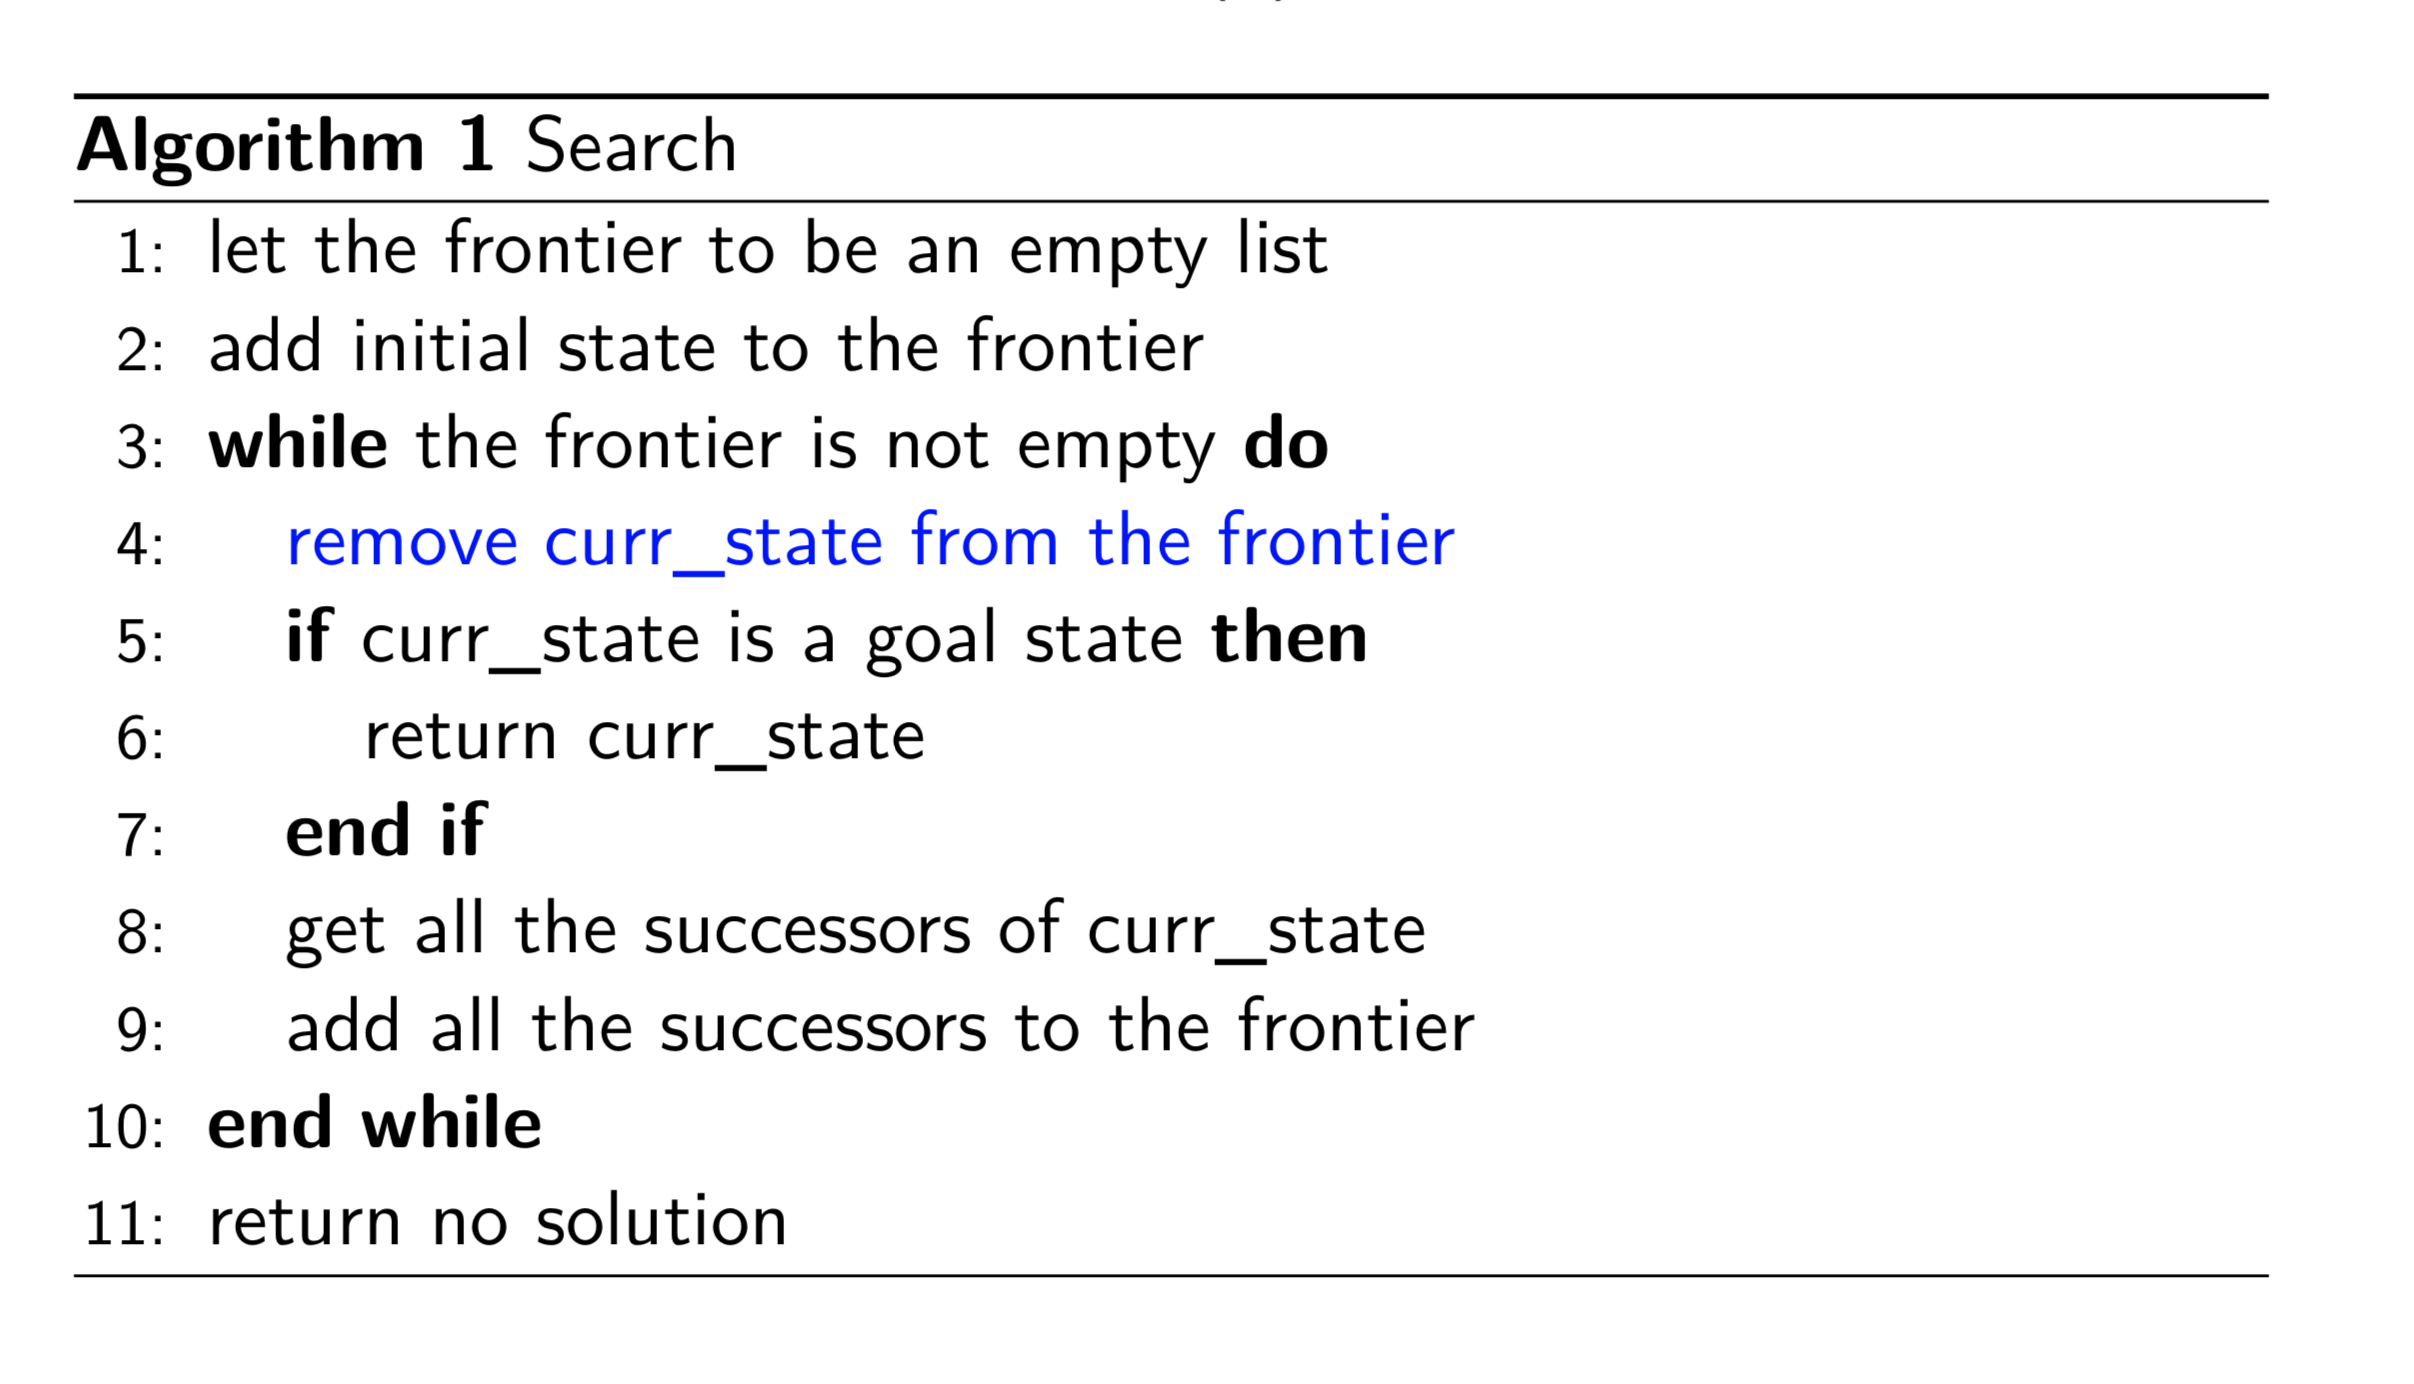
\includegraphics[scale=0.3]{1}
\end{center}

\end{document}





